\documentclass[11pt]{article}
\usepackage{subfigure,wrapfig,booktabs,fancyhdr,amsmath,amsfonts,float}
\usepackage[pdftex]{graphicx}
\usepackage{bm,amssymb,amsmath,amsthm,wasysym,color,fullpage,setspace,multirow}
\usepackage{listings}
\lstset{language=Matlab}

\newcommand{\vb}{\boldsymbol}
\newcommand{\vbh}[1]{\hat{\boldsymbol{#1}}}
\newcommand{\vbb}[1]{\bar{\boldsymbol{#1}}}
\newcommand{\vbt}[1]{\tilde{\boldsymbol{#1}}}
\newcommand{\vbs}[1]{{\boldsymbol{#1}}^*}
\newcommand{\vbd}[1]{\dot{{\boldsymbol{#1}}}}
\newcommand{\vbdd}[1]{\ddot{{\boldsymbol{#1}}}}
\newcommand{\by}{\times}
\newcommand{\tr}{{\rm tr}}
\newcommand{\cpe}[1]{\left[{#1} \times \right]}
\newcommand{\sfrac}[2]{\textstyle \frac{#1}{#2}}
\newcommand{\ba}{\begin{array}}
\newcommand{\ea}{\end{array}}
\renewcommand{\earth}{\oplus}
\newcommand{\sinc}{{\rm \hspace{0.5mm} sinc}}
\newcommand{\tf}{\tilde{f}}
\newcommand{\tbox}[1]{\noindent \fbox{\parbox{\textwidth}{#1}}}
\DeclareMathAlphabet{\mathpzc}{OT1}{pzc}{m}{it}

% Weird thing I have to add to allow `rubber` to compile
\DeclareUnicodeCharacter{2212}{-}

\title{ASE 389P-7 \\ Exam 2}
\author{Alejandro Moreno}\date{November 8, 2022}

\begin{document}
%\onehalfspace
\maketitle

\section{Problem 4}

\subsection{Instruction}

Download the gzipped archive \textbf{gridDataUt6.tar.gz} from
http://radionavlab.ae.utexas.edu/datastore/gnssSigProcCourse.
Un-zip and un-tar this file to get access to the underlying files. The
\textbf{*.log} files are columnar-format log files produced by the GRID receiver,
a powerful software-defined radionavigation receiver under development in the UT
Radionavigation Laboratory. The \textbf{*def.txt} files describe the data in the
corresponding \textbf{*.log} files. For now, you’ll only need to pay attention to
\textbf{channel.log}, whose format is described in \textbf{channeldef.txt}.
You’ll find that in this data set there were four L2C-capable GPS satellites
visible over the entire 27-minute data capture interval: those with TXIDs
(PRN identifiers) 7, 8, 19, and 28. For this data set, GRID tracked the signal
type GPS L1 CA on L1 and GPS L2 CL on L2. Draw the file \textbf{channel.log}
(or, equivalently, the file channel.mat) into Matlab and operate on the data to
generate a plot like the one shown in Figure 5.9 in the Misra and Enge textbook
for TXID 7. The plot should include both code- and carrier-derived ionospheric
delay time histories. Generate a second plot showing both the code- and
carrier-derived total electron content (TEC) seen by the signals from the
satellite with TXID 7. Express the value of TEC in TECU. Add a constant offset
to the carrier TEC so that it best matches the code TEC in a least-squares sense.

Answer the following questions:

\begin{itemize}
	\item What could explain the negative values in the final TEC estimates?
	      Is this physically possible?

	\item The ionospheric delay for TXID 7 changes significantly over the 27-minute
	      data capture interval. How is this possible if the GPS satellites move on
	      slow 12-sidereal-hour orbits? (You may wish to inspect the file
	      \textbf{navsol.log} for additional clues.)
\end{itemize}

\textbf{Hints:}\\


\begin{itemize}
	\item Make sure you match pseudorange and carrier phase measurements from the
	      L1 C/A signals with their L2 CL counterparts taken simultaneously.
	\item You’ll want to write a Matlab script to automate the process of drawing
	      in the data and generating the plots for this problem because you’ll
	      need to repeat the procedure in a later problem.
	\item The Matlab files *.mat contain the same data as the corresponding *.log
	      files but in a convenient Matlab format. The following Matlab command
	      sequence (1) draws channel.mat directly into Matlab, (2) stores the
	      contents of the file in the matrix M, (3) finds all the row indices
	      corresponding to the L1 C/A signal of the satellite with TXID 5,
	      (4) loads all the C/N0 measurements from these rows into C\_N0Vec\_txid05:

	      \begin{verbatim}
        >> load channel.mat
        >> M = channel’; // Transpose to get in columnar format
        >> iidum = find(M(:,13) == 0 & M(:,14) == 5);
        >> C_N0Vec_txid05 = M(iidum,9);
        \end{verbatim}
\end{itemize}


\subsection{Solution}

\subsubsection{Main function}

\begin{lstlisting}
  clc; close all; clear all;

  % Load the data
  load("gridDataUt6/channel.mat");
  M = channel';

  % Calculate the Ionopheric delay and plot it
  TXID = 7;
  N_L1 = 5609020;
  N_L2 = 5609020;
  [t, I_L1_code, I_L2_code, I_L1_carrier, I_L2_carrier] = ...
                              dualFreqIonoDelay(M, TXID, N_L1, N_L2);
  fig = plotIonoDelay(t, I_L1_code, 'code', NaN);
  fig = plotIonoDelay(t, I_L1_carrier, 'carrier', fig);
\end{lstlisting}

\subsubsection{Helper function}

\begin{lstlisting}
function [t, I_L1_code, I_L2_code, I_L1_carrier, I_L2_carrier] = ...
                                    dualFreqIonoDelay(M, TXID, N_L1, N_L2)
week2sec = 7 * 24 * 60 * 60;
c = physconst('LightSpeed');
f_L1 = 1575.42 * 1e6;
f_L2 = 1227.60 * 1e6;
lambda_L1 = c / f_L1;
lambda_L2 = c / f_L2;

GPS_L1_CA = 0;
GPS_L2_CL = 2;

% load L1
iidum = find(M(:,13) == GPS_L1_CA & M(:,14) == TXID &...
             M(:,3) ~= 9999 & M(:,10) == 1 & M(:,11) == 0);
ORT_week = M(iidum,3);
ORT_sec_week = M(iidum,4);
ORT_frac_sec = M(iidum,5);
t_L1 = week2sec*ORT_week + ORT_sec_week + ORT_frac_sec;
rho_L1 = M(iidum,8);
phi_L1 = M(iidum,7);

% load L2
iidum = find(M(:,13) == GPS_L2_CL & M(:,14) == TXID  &...
             M(:,3) ~= 9999 & M(:,10) == 1 & M(:,11) == 0);
ORT_week = M(iidum,3);
ORT_sec_week = M(iidum,4);
ORT_frac_sec = M(iidum,5);
t_L2 = week2sec*ORT_week + ORT_sec_week + ORT_frac_sec;
rho_L2 = M(iidum,8);
phi_L2 = M(iidum,7);

% Preprocess (IDK if the L1 and L2 samples coincide temporarly)
t0 = max(t_L1(1), t_L2(1));
tf = min(t_L1(end), t_L2(end));
t = linspace(t0, tf, 1e5);
rho_L1_intrp = spline(t_L1, rho_L1, t);
phi_L1_intrp = spline(t_L1, phi_L1, t);
rho_L2_intrp = spline(t_L2, rho_L2, t);
phi_L2_intrp = spline(t_L2, phi_L2, t);

% Ionospheric delay [Code]
I_L1_code = f_L2^2 / (f_L1^2 - f_L2^2) * (rho_L2_intrp - rho_L1_intrp);
I_L2_code = f_L1^2 / (f_L2^2 - f_L1^2) * (rho_L1_intrp - rho_L2_intrp);

% Ionospheric delay [Carrier]
I_L1_carrier = f_L2^2 / (f_L1^2 - f_L2^2) * ...
       (lambda_L1*(phi_L1_intrp - N_L1) - lambda_L2*(phi_L2_intrp - N_L2));
I_L2_carrier = f_L1^2 / (f_L2^2 - f_L1^2) * ...
       (lambda_L2*(phi_L2_intrp - N_L2) - lambda_L1*(phi_L1_intrp - N_L1));

end
\end{lstlisting}

\subsubsection{Results}

Figure~\ref{fig:ex4_iono_delay} shows the ionospheric delay calculated by
dual-frequency GPS.

\begin{figure}[H]
	\centering
	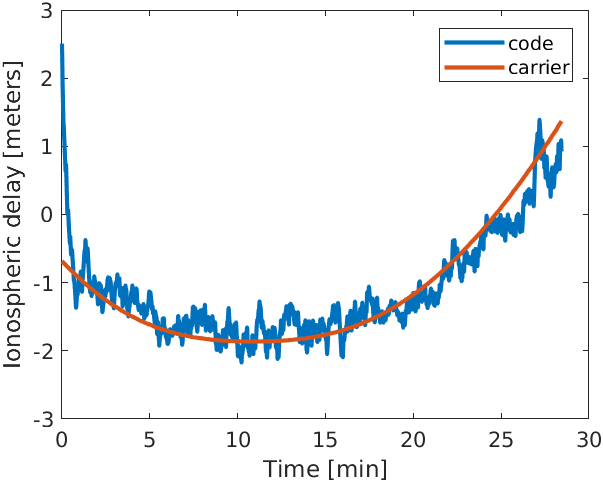
\includegraphics[width=0.9\textwidth]{figs/ex4_iono_delay.png}
	\caption{Ionospheric delay measured using code and carrier dual-frequency GPS.}
	\label{fig:ex4_iono_delay}
\end{figure}

The values shown in Figure~\ref{fig:ex4_iono_delay} are negative. This is not
physically possible. So, the must be related to some delay in the electronics
of the physical transmitter or receiver.

The rapid change in ionospheric delay could be due to the fact that the data
seems to be comming from a receiver in LEO orbit. This can be seen by analyzing
the navsol.log file. The height seem to vary from 100 to 600 km and the
velocity seems to range from 7500 to 8000 m/s. Knowing that Dr. Humphreys has a
receiver in the ISS I wouldn't be surprised if the data would be comming from
there. Thus, the rapid movement of the receiver through the ionosphere explains
the fast fluctuation of ionospheric delay.

\section{Problem 5}

\subsection{Instruction}

Write a function in Matlab for computing the ionospheric delay from a model of
the ionosphere. Your function should adhere to the interface described on the
next page (which you can copy and paste as comments to your function). Only
develop calculations for the broadcast (Klobuchar) model. The function can later
be augmented to accommodate other model types. You can learn about the broadcast
model on pages 168-169 of the Misra and Enge text. More details can be found on
pages 128-130 of the GPS interface specification (IS) IS-GPS-200F.pdf posted on
Canvas. You will also need to write your own function for computing satellite
elevation and azimuth angles. Assume the WGS84 model for the shape of the Earth.
Note that the GPS IS uses semicircles as its angular measure, which is a strange
convention employed back in the 1970s to reduce memory and computation
requirement. The sin and cos functions in the IS (e.g., in Fig. 20-4) are meant
to operate on semicircles, unless otherwise indicated. Thus, when the IS writes,
e.g., $cos(\lambda_i −1.1617)$, where $\lambda_i$ is given in semicircles, you
can implement this in Matlab as $cos((\lambda_i −1.1617)\pi)$.

\subsection{Solution}


\begin{lstlisting}
function [delTauG] = getIonoDelay(ionodata,fc,rRx,rSv,tGPS,model)
% getIonoDelay : Return a model-based estimate of the ionospheric delay
%                experienced by a trans-ionospheric GNSS signal as it
%                propagates from a GNSS SV to the antenna of a terrestrial
%                GNSS receiver.
%
% INPUTS
%
% ionodata ------- Structure containing a parameterization of the
%                  ionosphere that is valid at time tGPS. The structure is
%                  defined differently depending on what ionospheric model
%                  is selected:
%
%                  broadcast --- For the broadcast (Klobuchar) model, ionodata
%                                is a structure containing the following fields:
%
%                       alpha0 ... alpha3 -- power series expansion coefficients
%                                            for amplitude of ionospheric delay
%                       beta0 ... beta3 -- power series expansion coefficients
%                                          for period of ionospheric plasma density 
%                                          cycle
%
%
% Other models TBD ...
%
% fc ------------- Carrier frequency of the GNSS signal, in Hz.
%
% rRx ------------ A 3-by-1 vector representing the receiver antenna position
%                  at the time of receipt of the signal, expressed in meters
%                  in the ECEF reference frame.
%
% rSv ------------ A 3-by-1 vector representing the space vehicle antenna
%                  position at the time of transmission of the signal,
%                  expressed in meters in the ECEF reference frame.
%
% tGPS ----------- A structure containing the true GPS time of receipt of
%                  the signal. The structure has the following fields:
%                  week -- unambiguous GPS week number
%                  seconds -- seconds (including fractional seconds) of the
%                  GPS week
%
% model ---------- A string identifying the model to be used in the
%                  computation of the ionospheric delay:
%                  broadcast --- The broadcast (Klobuchar) model.
%
% Other models TBD ...
%
% OUTPUTS
%
% delTauG -------- Modeled scalar excess group ionospheric delay experienced
%                  by the transionospheric GNSS signal, in seconds.
%
%+----------------------------------------------------------------------------+
% References: For the broadcast (Klobuchar) model, see IS-GPS-200F
% pp. 128-130.
%
%+============================================================================+
wgs84 = wgs84Ellipsoid('meter');
[lat,lon,h] = ecef2geodetic(wgs84, rRx(1), rRx(2), rRx(3));
[az,elev,slantRange] = ecef2aer(rSv(1), rSv(2), rSv(3), lat, lon, h, wgs84);
lambda_u = lon/180; % user geodetic longitude (semi-circles)
phi_u    = lat/180; % user geodetic latitude (semi-circles) 
A        = az/180;  % azimuth angle between user and satellite, measured clockwise 
                % positive from the true North (semi-circles) 
E        = elev/180;% elevation angle between user and satellite (semi_circle)

% earth's  central  angle  between  the  user  position  and  the  earth  
% projection  of ionospheric intersection point (semi-circles) 
Psi = 0.0137/(E+0.11) - 0.022;

% geodetic  latitude  of  the  earth  projection  of  the  ionospheric  
% intersection  point (semi-circles) 
phi_i = phi_u + Psi * cos(A*pi);
phi_i = max(-0.416, phi_i);
phi_i = min(0.416, phi_i);

% geodetic  longitude  of  the  earth  projection  of  the  ionospheric  
% intersection  point (semi-circles) 
lambda_i = lambda_u + Psi*cos(A*pi)/cos(phi_i*pi);

% geomagnetic latitude of the earth projection of the ionospheric 
% intersection point (mean ionospheric height assumed 350 km) (semi-circles) 
phi_m = phi_i + 0.064*cos((lambda_i - 1.617)*pi);

% local time (sec) 
t = 4.32*(10^4)*lambda_i + tGPS.seconds;
while t > 86400
    t = t - 86400;
end
while t < 0
    t = t + 86400;
end

PER = ionodata.broadcast.beta0 * phi_m^0 + ...
      ionodata.broadcast.beta1 * phi_m^1 + ...
      ionodata.broadcast.beta2 * phi_m^2 + ...
      ionodata.broadcast.beta3 * phi_m^3;
PER = max(72000, PER);


AMP = ionodata.broadcast.alpha0 * phi_m^0 + ...
      ionodata.broadcast.alpha1 * phi_m^1 + ...
      ionodata.broadcast.alpha2 * phi_m^2 + ...
      ionodata.broadcast.alpha3 * phi_m^3;
AMP = max(0, AMP);

% phase (radians) 
x = 2*pi*(t - 50400)/PER;

% obliquity factor (dimensionless) 
F = 1 + 16*(0.53 - E)^3;

% Estimate the ionospheric delay
if abs(x) < 1.57
    T_iono = F*(5e-9 + AMP * (1 - (x^2)/2 + (x^4)/24));
else
    T_iono = F * 5e-9;
end

if fc == 1227.44 * 1e6
    gamma = (77/60)^2;
    T_iono = gamma * T_iono;
end

delTauG = T_iono;
end
\end{lstlisting}

\subsection{Results}

The solution I got for the conditions provided was $delTauG = 23.3269 ns$, which
translates to about 7 meters.

\section{Problem 5}

\subsection{Code}


\begin{lstlisting}
function [IVec,QVec] = if2iq(xVec,T,fIF)
% IF2IQ : Convert intermediate frequency samples to baseband I and Q samples.
%
% Let x(n) = I(n*T)*cos(2*pi*fIF*n*T) - Q(n*T)*sin(2*pi*fIF*n*T) be a
% discrete-time bandpass signal centered at the user-specified intermediate
% frequency fIF, where T is the bandpass sampling interval. Then this
% function converts the bandpass samples to quadrature samples from a complex
% discrete-time baseband representation of the form xl(m*Tl) = I(m*Tl) +
% j*Q(m*Tl), where Tl = 2*T.
%
%
% INPUTS
%
% xVec -------- N-by-1 vector of intermediate frequency samples with
%               sampling interval T.
%
% T ----------- Sampling interval of intermediate frequency samples, in
%               seconds.
%
% fIF --------- Intermediate frequency of the bandpass signal, in Hz.
%
%
% OUTPUTS
%
% IVec -------- N/2-by-1 vector of in-phase baseband samples.
%
% QVec -------- N/2-by-1 vector of quadrature baseband samples.
%
%
%+------------------------------------------------------------------------------+
% References:
%
%
%+==============================================================================+
n = 0:1:length(xVec)-1; n=n';
IVec = 2*cos(2*pi*fIF*n*T).*xVec;
QVec = -2*sin(2*pi*fIF*n*T).*xVec; % figure out the sign

IVec = decimate(IVec,2)/sqrt(2);
QVec = decimate(QVec,2)/sqrt(2);
\end{lstlisting}


\begin{lstlisting}
function [xVec] = iq2if(IVec,QVec,Tl,fIF)
% IQ2IF : Convert baseband I and Q samples to intermediate frequency samples.
%
% Let xl(m*Tl) = I(m*Tl) + j*Q(m*Tl) be a discrete-time baseband
% representation of a bandpass signal. This function converts xl(n) to a
% discrete-time bandpass signal x(n) = I(n*T)*cos(2*pi*fIF*n*T) -
% Q(n*T)*sin(2*pi*fIF*n*T) centered at the user-specified intermediate
% frequency fIF, where T = Tl/2.
%
%
% INPUTS
%
% IVec -------- N-by-1 vector of in-phase baseband samples.
%
% QVec -------- N-by-1 vector of quadrature baseband samples.
%
% Tl ---------- Sampling interval of baseband samples (complex sampling
%               interval), in seconds.
%
% fIF --------- Intermediate frequency to which the baseband samples will
%               be up-converted, in Hz.
%
%
% OUTPUTS
%
% xVec -------- 2*N-by-1 vector of intermediate frequency samples with
%               sampling interval T = Tl/2.
%
%
%+------------------------------------------------------------------------------+
% References:
%
%
%+==============================================================================+
IVec_resampled = interp(IVec,2);
QVec_resampled = interp(QVec,2);

T = Tl/2;
n = 0:1:length(IVec_resampled)-1; n=n';
xVec = IVec_resampled.*cos(2*pi*fIF*n*T) ...
        - QVec_resampled.*sin(2*pi*fIF*n*T);

xVec = sqrt(2)*xVec;
\end{lstlisting}

\subsection{Results}

The power spectral density of the original signal (baseband representation),
the bandpass representation and the reconstructed baseband representation can
be observed in Figures~\ref{fig:ex5_baseband_original}, \ref{fig:ex5_bandpass}
and \ref{fig:ex5_baseband_reconstructed}, respectively. Note that the bandpass
representation had to be centered at a $f_{IF} = 5MHz$ to be able to reconstruct
the signal without distortion since the bandwidth of the original signal is
approximately 5MHz.

\begin{figure}[H]
	\centering
	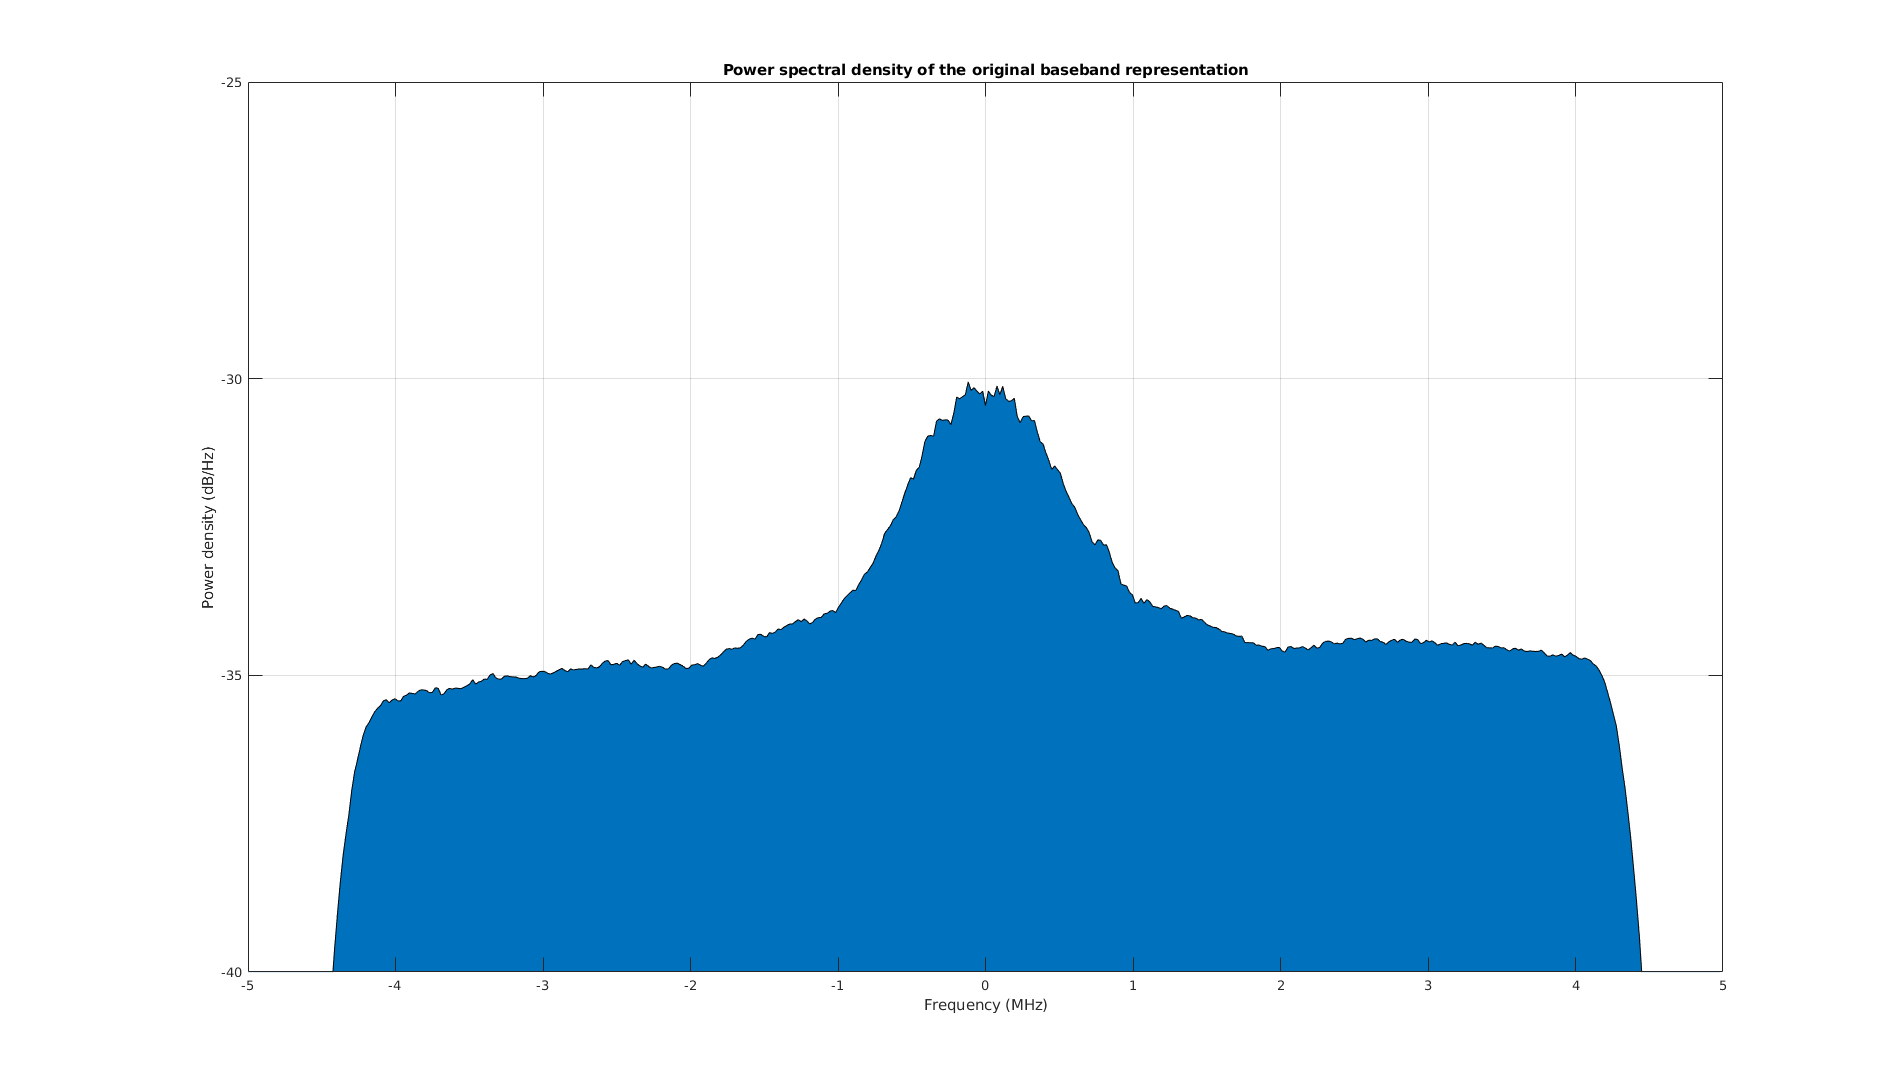
\includegraphics[width=0.9\textwidth]{figs/PSD_baseband_original.png}
	\caption{Power spectral density of the original signal in its baseband
		representation.}
	\label{fig:ex5_baseband_original}
\end{figure}

\begin{figure}[H]
	\centering
	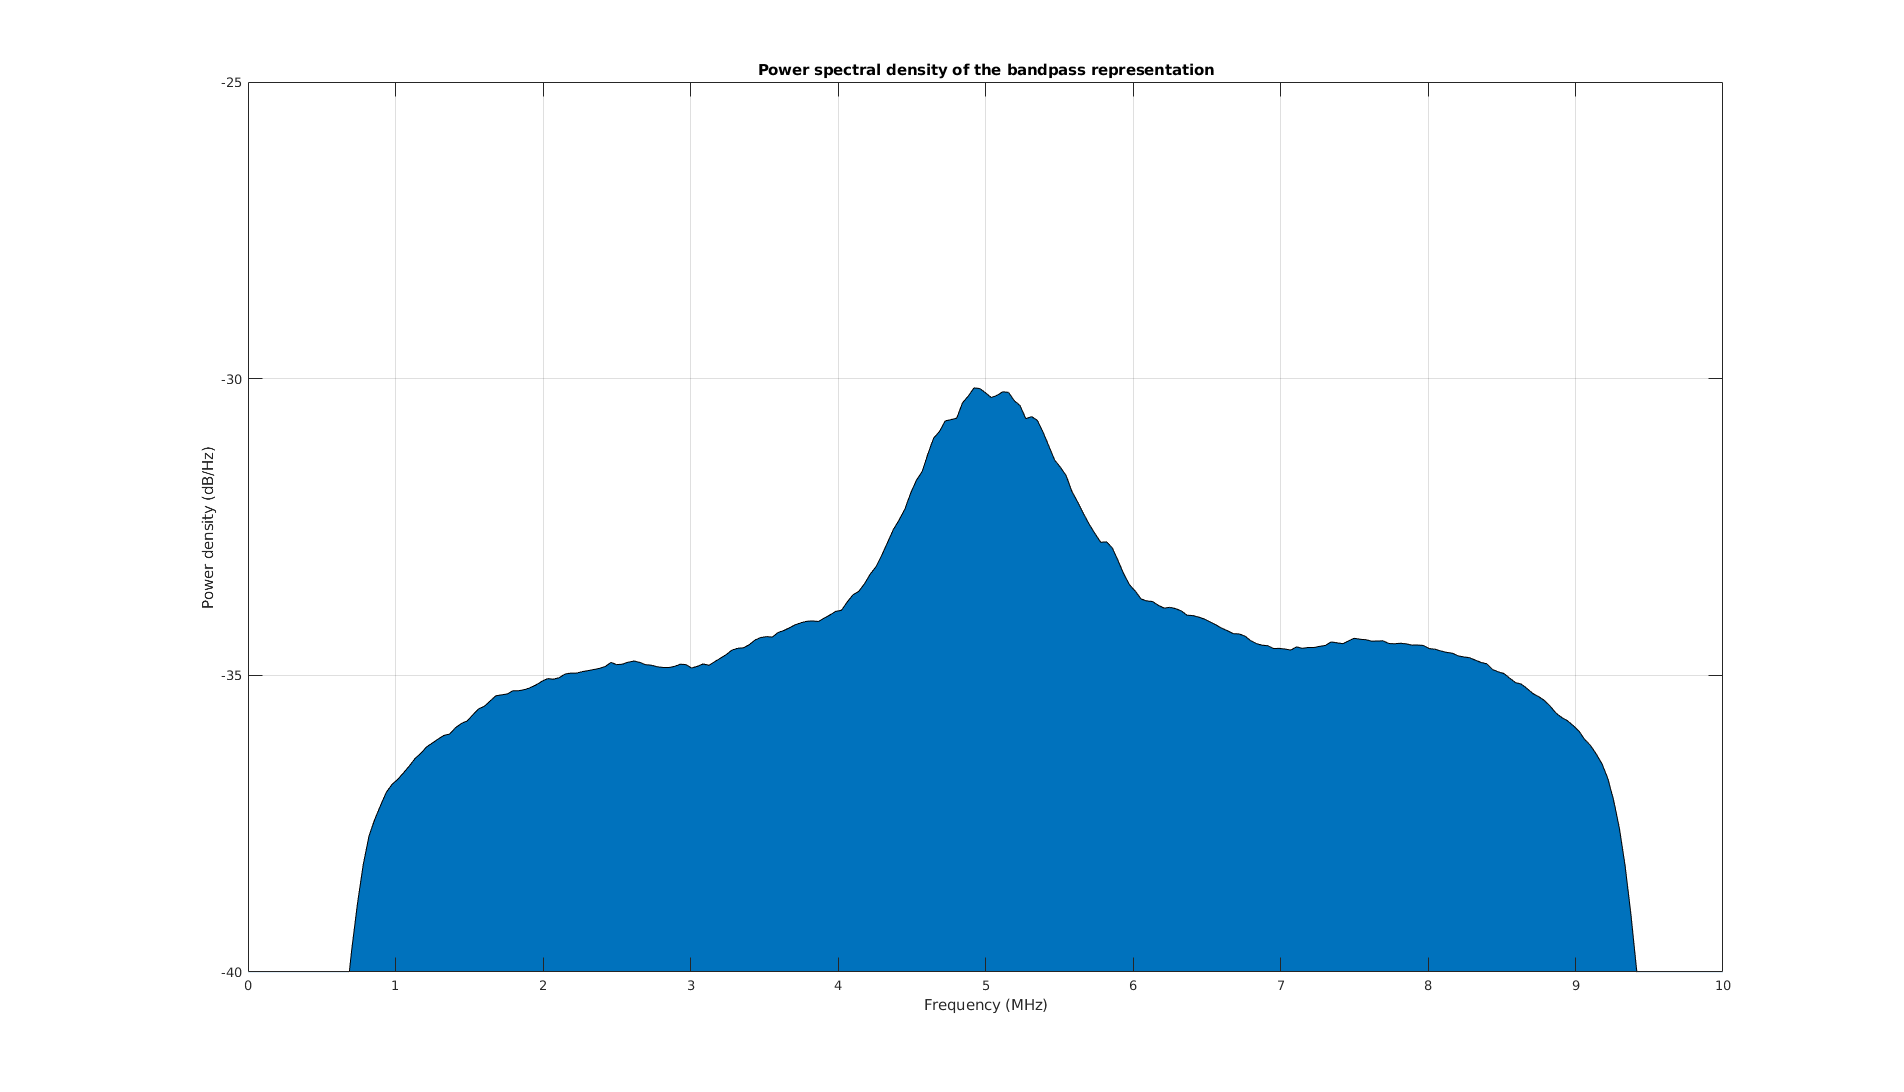
\includegraphics[width=0.9\textwidth]{figs/PSD_bandpass.png}
	\caption{Power spectral density of the bandpass representation of the original
		signal.}
	\label{fig:ex5_bandpass}
\end{figure}

\begin{figure}[H]
	\centering
	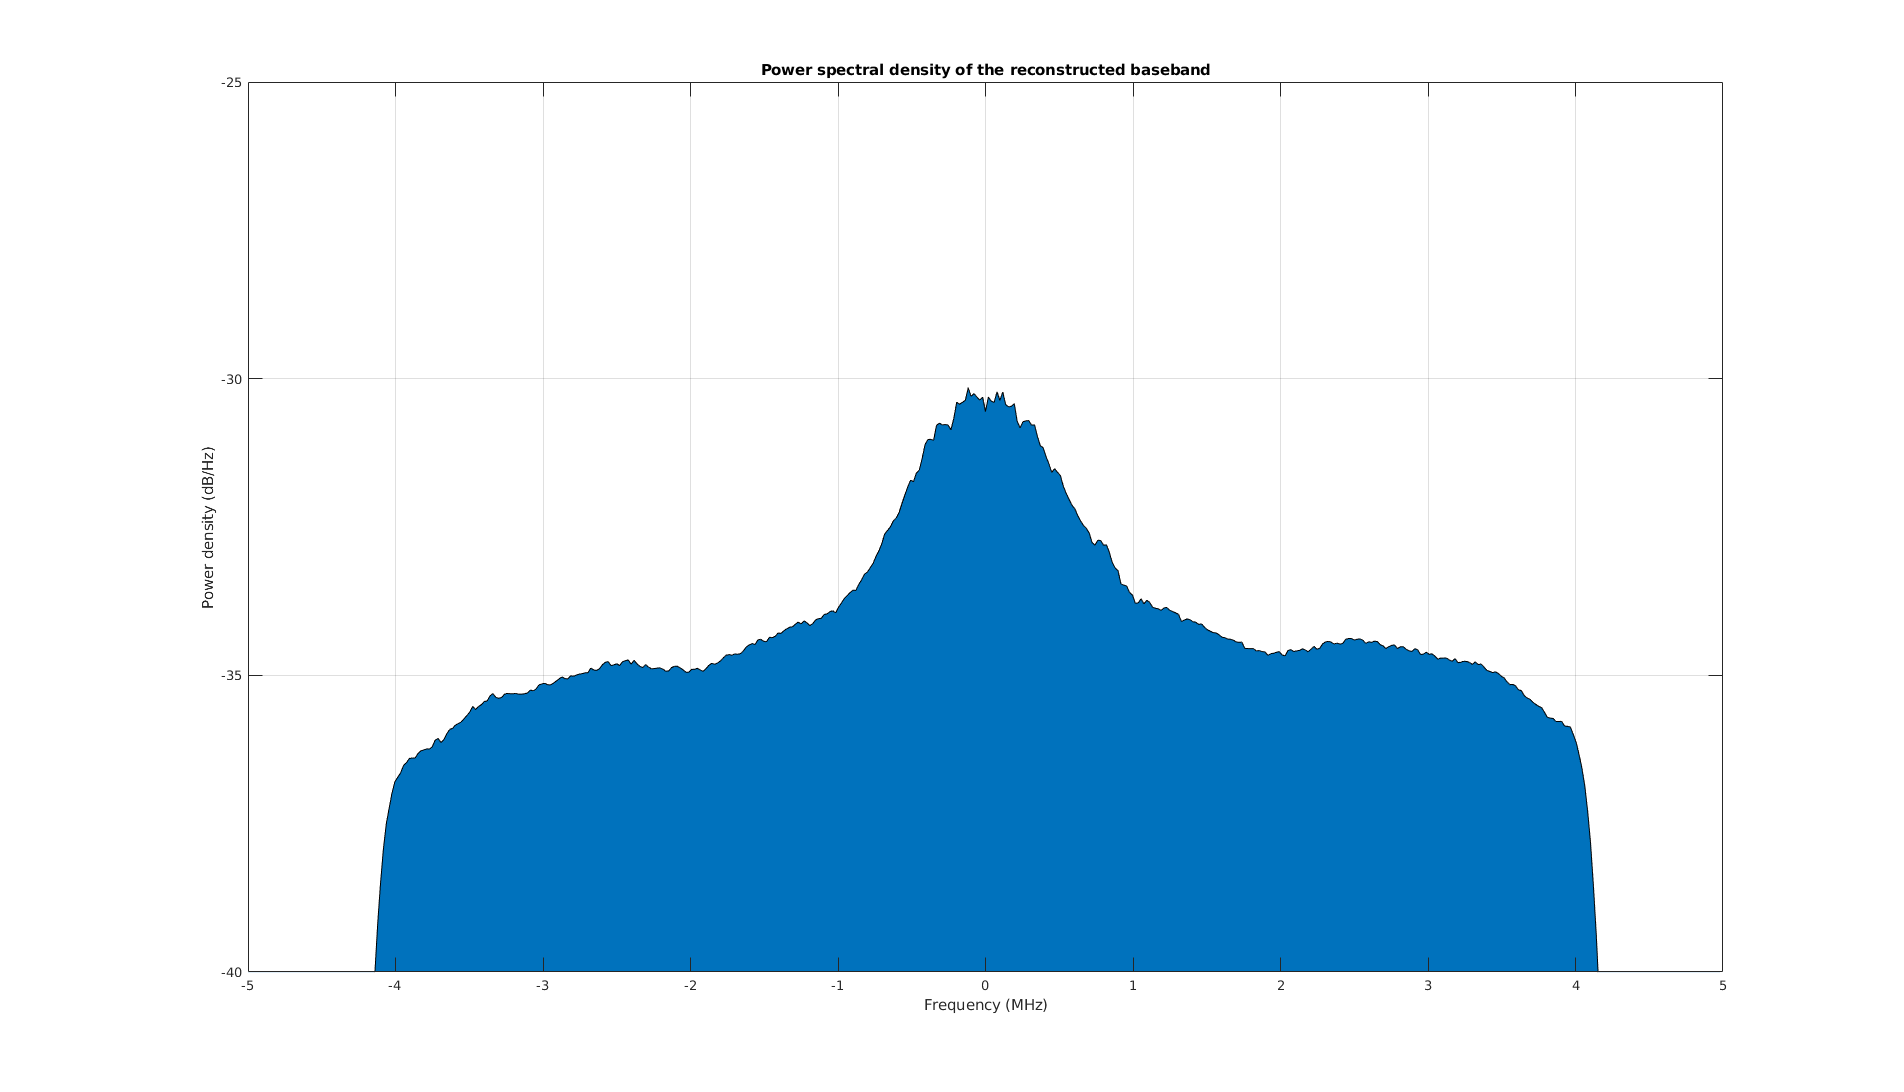
\includegraphics[width=0.9\textwidth]{figs/PSD_baseband_reconstructed.png}
	\caption{Power spectral density of the reconstructed signal in its baseband
		representation.}
	\label{fig:ex5_baseband_reconstructed}
\end{figure}

It can it seen from the graphs that the manipulation of the original signal
by processing it with the functions \textbf{iq2if} and \textbf{if2iq} slightly
changes the PSD, it makes it smoother. This is consistent with the fact that
these functions internally apply a low pass filter and therefore some of the
edges end up a little bit more rounded than originally.

\section{Problem 8}

\subsection{Code}

\begin{lstlisting}
clc; clear all; close all; format long g;
%----- Setup
Tfull = 0.5;     % Time interval of data to load
fs = (40/7)*1e6; % IQ sampling frequency (Hz)
Ts = 1/fs;
N = floor(fs*Tfull/16)*16;
nfft = 2^9;      % Size of FFT used in power spectrum estimation
%----- Load data
fileName = 'dataout_raw_trimmed_158.bin';
fid = fopen(fileName,'r','l');
[yhist,count] = binloadSamples(fid,N,'dual');
yhist = yhist(:,1);
fclose(fid);

%----- Compute power spectrum estimate
[Syy,fVec] = pwelch(yhist,hann(nfft),[],nfft, fs);
plotPSD(Syy, fVec, nfft, fs, -63, -55);

% Convert signal to its baseband representation and compute PSD
fIF = 1610476.187;
[IVec,QVec] = if2iq(yhist, Ts, fIF);
xVec = IVec + j*QVec;
[Syy_IQ, fVec_IQ] = pwelch(xVec,hann(nfft),[],nfft, fs/2);
plotPSD(Syy_IQ, fVec_IQ, nfft, fs, -63, -55);

tau = (Ts*2)*(0:1:N-1)'; % sampling time (in RX time base)

fStep = 10; % Hz
nStep = 1;  % Ts
for TXID = 1:37
    [fDk_hat(TXID), tsk_hat(TXID), C_N0_hat(TXID), detected(TXID)] = 
                    acquireGPS(tau, xVec, Ts*2, 5, fStep, nStep, TXID, 'FFT');
end
\end{lstlisting}

\begin{lstlisting}
%%%%%%%%%%%%%%%%%%%%%%%%%%%%%%%%%%%%%%%%%%%%%%%%%%%%%%%%%%%%%%%%%%%%%%%%%%%%%%%%
function [fdk_hat, tsk_hat, C_N0, isAcquired] = acquireGPS(tau, x, T, nTc,...
                                                fStep, nStep, TXID, method)
% Spreading code replica
Nc = 1023;
Tc = 1e-3/Nc;
code = generatePRN(TXID); 

% generate data for the k-th accumulation 
Ta = nTc*Nc*Tc;
Nk = floor(Ta/T);
tau = tau(1:Nk);
x   = x(1:Nk);

% resample C at TsamplingIQ
code = repmat(code, [nTc 1] );
C = oversampleSpreadingCode(code, T/Tc, 0, Nk, Nc);

epsilon = 50*(nTc/Ta);
fDk_hat = -epsilon:fStep:epsilon;
M = zeros(Nk,length(fDk_hat));
if strcmp(method, 'FFT')
    Cr = fft(C);
    parfor fDk_idx = 1:length(fDk_hat)
        % phase estimate over the accumulation interval
        theta_jk_hat = 0;
        theta_hat = 2*pi*fDk_hat(fDk_idx)*tau + theta_jk_hat;

        x_tilde = x.*exp(-i*theta_hat);
        Xr_tilde = fft(x_tilde);
        Zr = Xr_tilde.*conj(Cr);
        zk = ifft(Zr);
        
        M(:,fDk_idx) = abs(zk).^2;
    end
else
    parfor fDk_idx = 1:length(fDk_hat)
        for n = 1:nStep:Nk            
            % phase estimate over the accumulation interval
            theta_jk_hat = 0;
            theta_hat = 2*pi*fDk_hat(fDk_idx)*tau + theta_jk_hat;
            
            % Align C with the code in the incoming data.
            Cshift = circshift(C,n-1);

            % Calculate Sk and store in a matrix that represents the 2D-grid
            Sk = sum(x.*exp(-i*(theta_hat)).*Cshift);
            M(n, fDk_idx) = abs(Sk)^2;
        end
    end
end

% % DEBUG
% tau_jk = tau(1:Nk)*1e6;
% ii = find(tau_jk<1000);
% figure();
% h = surf(fDk_hat, tau_jk(ii), M(ii,:));
% set(h,'LineStyle','none')
% title('2D grid - S_k')
% xlabel('$\hat{f}_{Dk} [Hz]$','Interpreter','latex')
% ylabel('$\tau_{jk} [us]$','Interpreter','latex')

% Find the maximum Sk in the 2D-grid
[max_Sk, max_idx] = max(M(:));
[n, fDk_idx]=ind2sub(size(M),max_idx);

% Estimates
isAcquired = max_Sk > 1.5e6;
fdk_hat = fDk_hat(fDk_idx); % Hz
tsk_hat = tau(n)*1e6;       % us 

two_sigmaIQ_squared = 61551.7110161536; % mean(M,'all') for satellite 34
%two_sigmaIQ_squared = 568409076.119826; % mean(M,'all') for satellite 34
C_N0 = 10*log10((max_Sk - two_sigmaIQ_squared)/(two_sigmaIQ_squared*Ta));

end
%%%%%%%%%%%%%%%%%%%%%%%%%%%%%%%%%%%%%%%%%%%%%%%%%%%%%%%%%%%%%%%%%%%%%%%%%%%%%%%
\end{lstlisting}


\subsection{Results}

\begin{tabular}{c|c|c|c}
	PRN & Doppler [MHz] & $\tau$ [$\mu s$] & C/N0   \\
	\hline
	1   & $-33.840$     & 410              & $48$   \\
	11  & $-35.910$     & 578              & $48.9$ \\
	14  & $-20.280$     & 35               & $38.8$ \\
	18  & $-34.220$     & 370              & $50$   \\
	31  & $-25.350$     & 804              & $40.9$ \\
\end{tabular}


\begin{figure}[H]
	\centering
	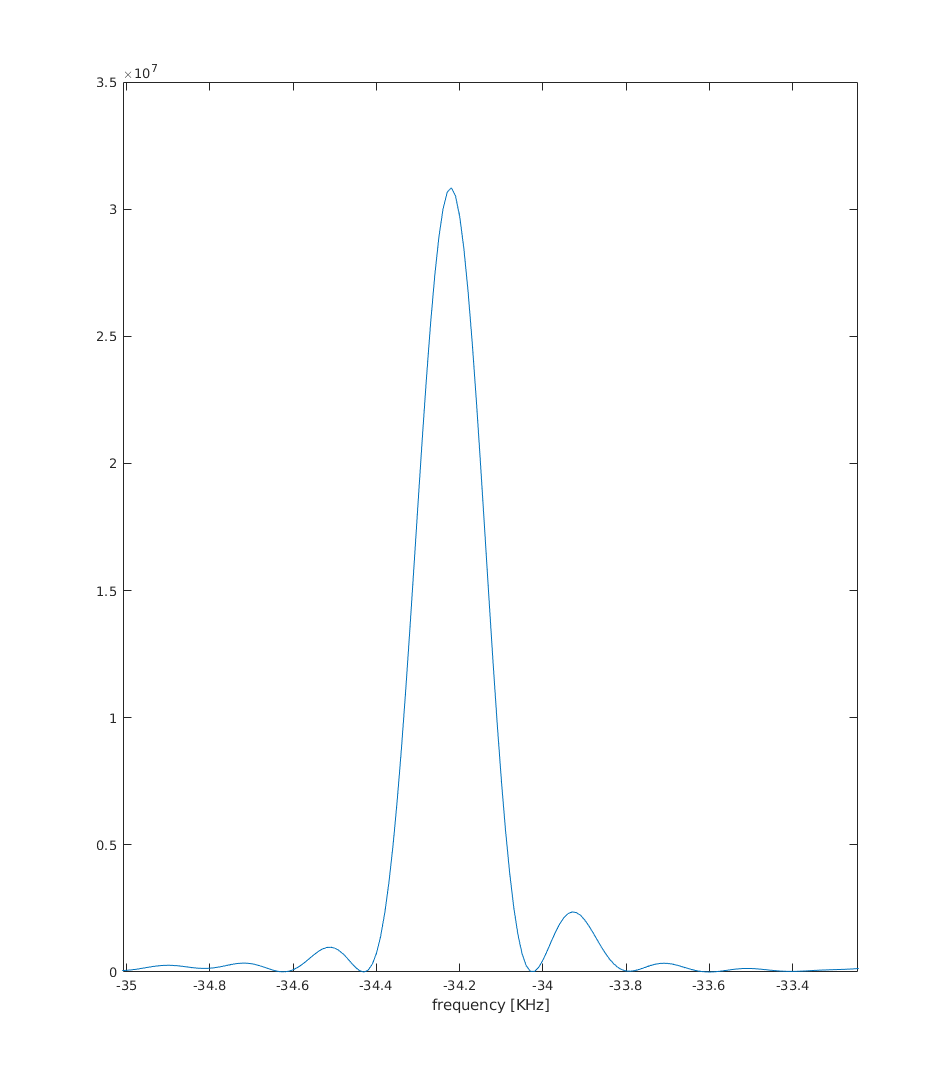
\includegraphics[width=0.9\textwidth]{figs/Sk_freq.png}
	\caption{$|S_k| vs \hat{f}_{D,k}$ for the maximizing $\hat{t}_{s,k}$.}
	\label{fig:sk_freq}
\end{figure}

\begin{figure}[H]
	\centering
	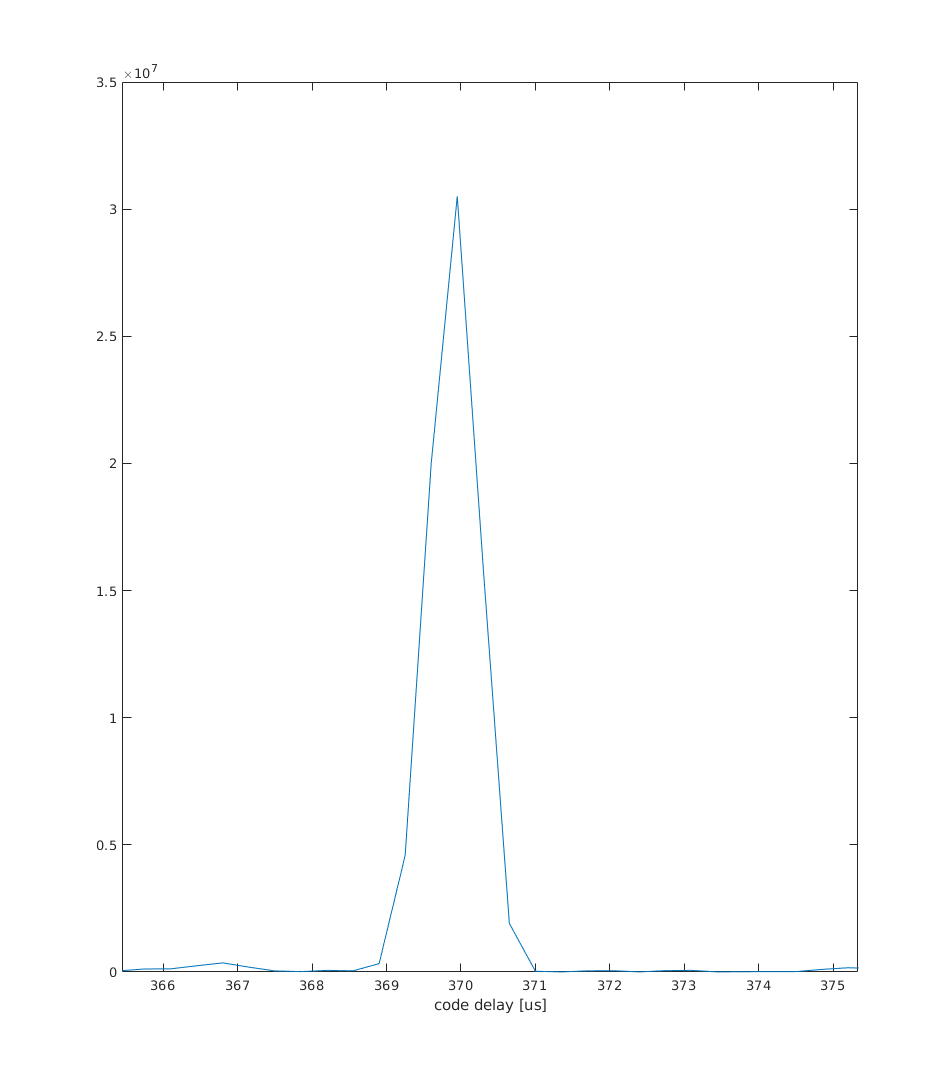
\includegraphics[width=0.9\textwidth]{figs/Sk_tau.png}
	\caption{$|S_k| vs \hat{t}_{s,k}$ for the maximizing $\hat{f}_{D,k}$.}
	\label{fig:sk_tau}
\end{figure}

\section{Problem 8}

\subsection{Code}

\begin{lstlisting}
function [pZ_H0,pZ_H1,lambda0,Pd,ZVec] = performAcqHypothesisCalcs(s)
% performAcqHypothesisCalcs : Calculate the null-hypothesis and alternative
%                             hypothesis probability density functions and 
%                             the decision threshold corresponding to GNSS 
%                             signal acquisition with the given inputs.
%
% Z is the acquisition statistic:
%
%        N  |    |^2
% Z =   sum | Sk |
%       k=1 |    |
%
%
%
%      N   |             |
%   = sum  | Ik^2 + Qk^2 |
%     k=1  |             |
%
%
%
% where Sk = rhok + nk = Ik + j*Qk
%
% and nk = nIk + j*nQk
%
% with nIk ~ N(0,1), nQk ~ N(0,1), and E[nIk nQi] = 1 for k = i and 0 for k !=
% i. The amplitude rhok is related to familiar parameters Nk, Abark, and
% sigma_IQ by rhok = (Nk*Abark)/(2*sigma_IQ), i.e., it is the magnitude of the
% usual complex baseband phasor normalized by sigma_IQ.
%
% Under H0, the statistic Z is distributed as a chi square distribution with
% 2*N degrees of freedom; under H1, it is distributed as a noncentral chi
% square distribution with lambda = N*rhok^2 and 2*N degrees of freedom.
%
% The total number of cells in the search grid is assumed to be nCells =
% nCodeOffsets*nFreqOffsets, where nFreqOffsets = 2*fMax*Ta and Ta = Na*T is
% the total coherent accumulation time. Here, Na is the average value of the
% number of samples in each accumulation, Nk.
%
% INPUTS
%
% s -------- A structure containing the following fields:
%
% C_N0dBHz ------- Carrier to noise ratio in dB-Hz.
%
% Ta ------------- Coherent accumulation interval, in seconds.
%
% N -------------- The number of accumulations summed noncoherently to
%                  get Z.
%
% fMax ----------- Frequency search range delimiter. The total
%                  frequency search range is +/- fMax.
%
% nCodeOffsets --- Number of statistically independent code offsets in
%                  the search range.
%
% PfaAcq --------- The total acquisition false alarm probability.
%                  This is the probability that the statistic Z
%                  exceeds the threshold lambda in any one of the
%                  search cells under the hypothesis H0. One can
%                  derive the false alarm probability for *each*
%                  search cell from PfaAcq. This procedure is
%                  straightforward if we assume that the detection
%                  statistics from the search cells are independent
%                  of one another.
%
% ZMax ----------- The maximum value of Z that will be considered.
%
% delZ ----------- The discretization interval used for the
%                 independent variable Z. The full vector of Z
%                 values considered is thus ZVec = [0:delZ:ZMax].
%
%
% OUTPUTS
%
% pZ_H0 ---------- The probability density of Z under hypothesis H0.
%
% pZ_H1 ---------- The probability density of Z under hypothesis H1.
%
% lambda0 -------- The detection threshold.
%
% Pd ------------- The probability of detection.
%
% Zvec ----------- The vector of Z values considered.
%
%+------------------------------------------------------------------------+
% References:
%
%
%+========================================================================+
dof = 2*s.N;
ZVec = 0:s.delZ:s.ZMax;
nFreqOffsets = 2*s.fMax*s.Ta;
nCells = s.nCodeOffsets * nFreqOffsets;
rho_squared = 10^(s.C_N0dBHz/10) * 2 * s.Ta;
lambda = s.N * rho_squared;

% compute the probability density of Z under hypothesis H0 and H1
pZ_H0 = chi2pdf(ZVec, dof)';
pZ_H1 = ncx2pdf(ZVec, dof, lambda)';

% Calculate the threshold that ensures that the probability of false 
% acquisition is below the user-defined value
Pf = 1 - (nthroot((1-s.PfaAcq), nCells));
nuStar = chi2inv(1-Pf, dof);
lambda0 = nuStar;

% Calculate the probability of detection
Pd = 1 - ncx2cdf(nuStar, dof, lambda);
\end{lstlisting}


\subsection{Results}

\subsubsection{Part A}

In part A, N was adjusted to reach a probability of detection in the neighborhood
of 95\% for signals with different carrier-to-noise ratios, this is shown in
Figure~\ref{fig:pd_vs_N}.

\begin{figure}[H]
	\centering
	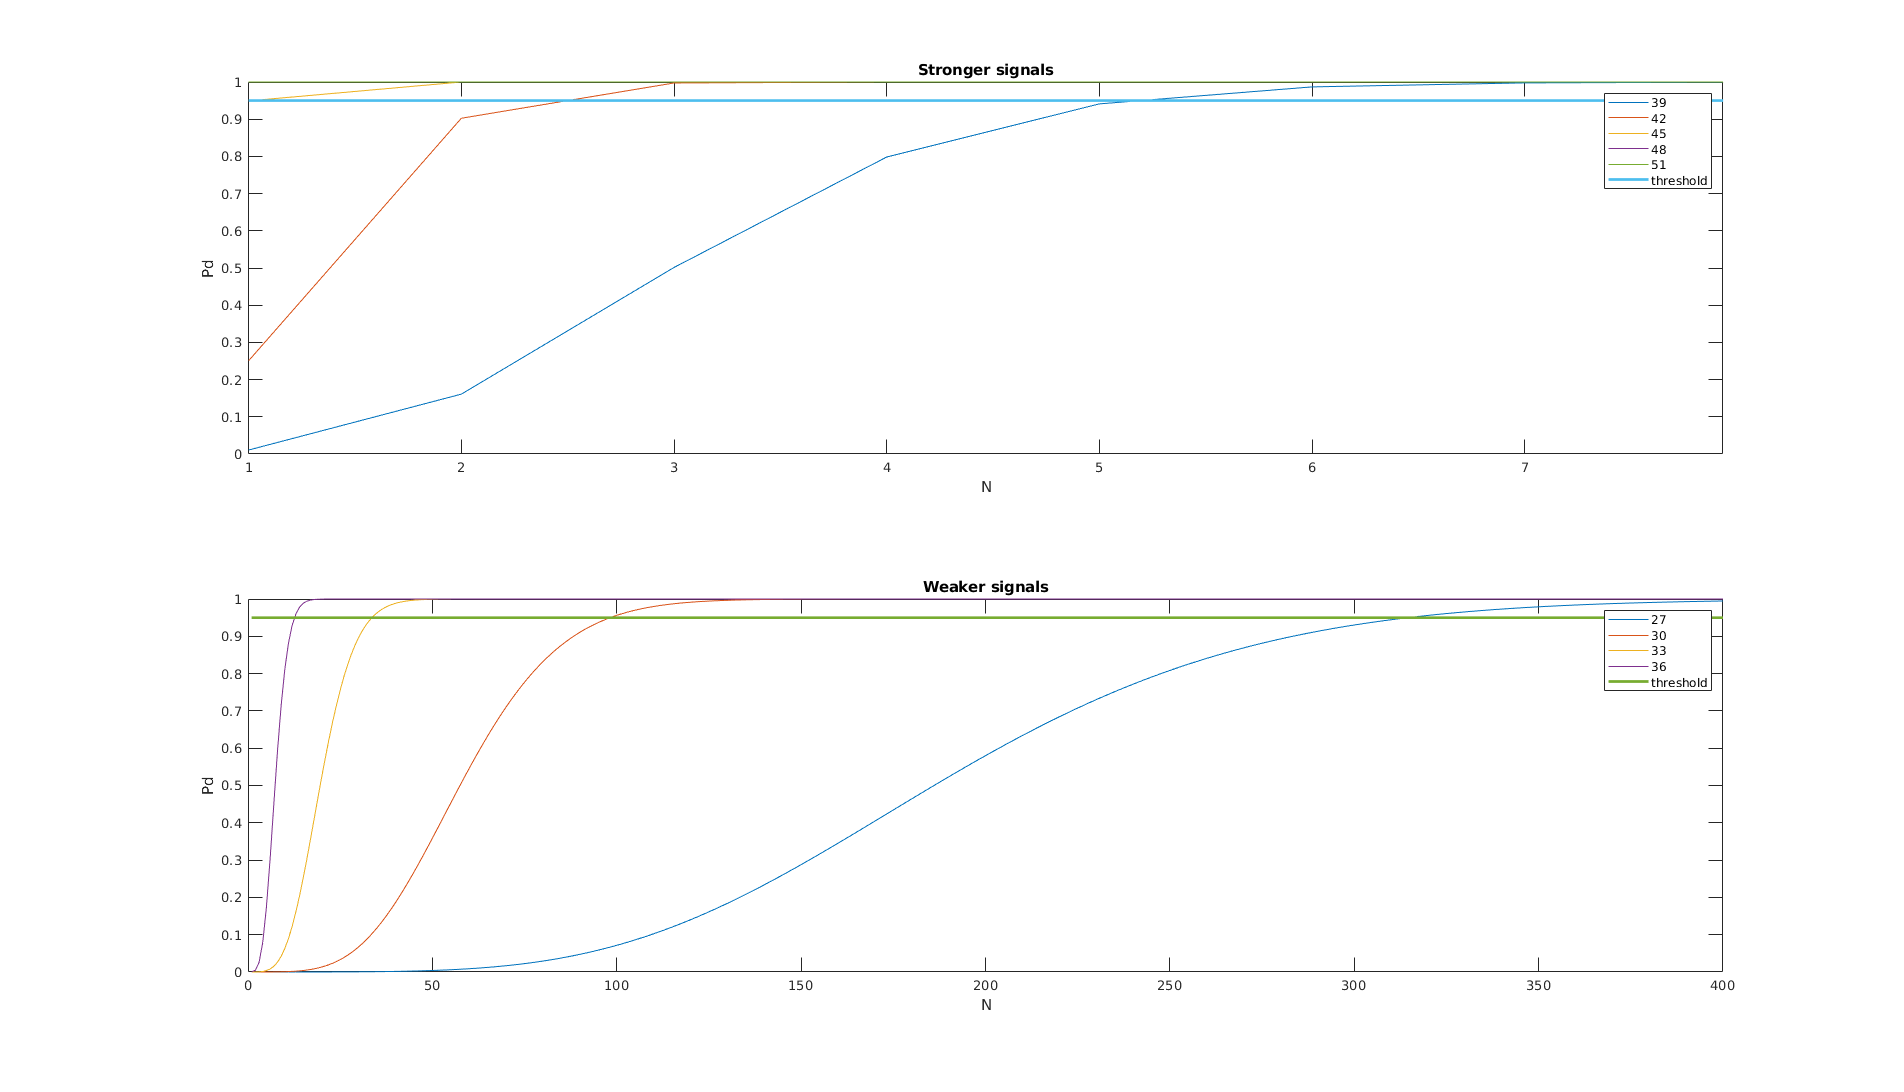
\includegraphics[width=0.9\textwidth]{figs/Pd_vs_N.png}
	\caption{Probability of detection vs. number of accumulation periods for
		different C/N0 ratios (Non-coherent accumulation).}
	\label{fig:pd_vs_N}
\end{figure}

In Figure~\ref{fig:HT_partA_30dBHz} it is possible to observe a particular case
of the hypothesis testing for GNSS acquisition. In particular, it is taylored
to detect a 30dBHz C/N0 signal with 95\% probability and 0.01\% chance of false
alarm by performing non-coherent integration.

\begin{figure}[H]
	\centering
	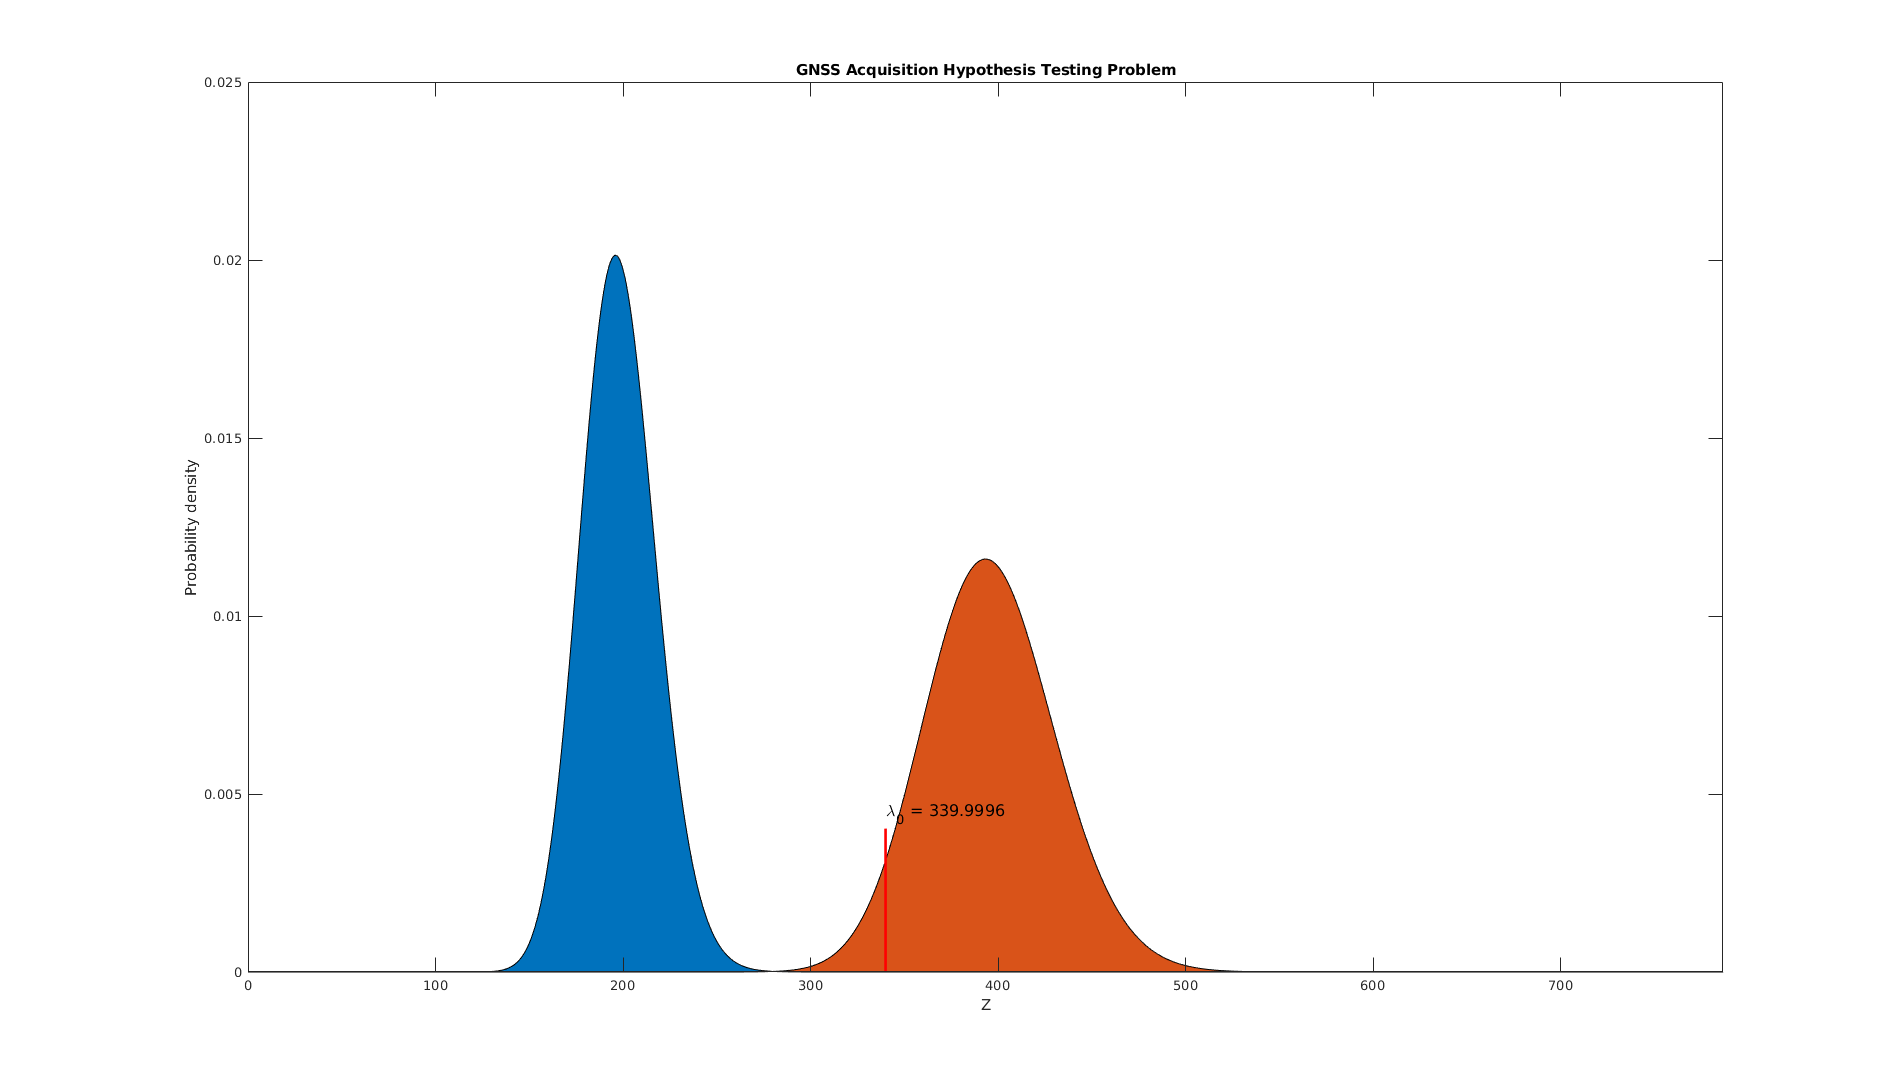
\includegraphics[width=0.9\textwidth]{figs/HT_partA_30dBHz.png}
	\caption{Hypothesis testing for the case where a 30dBHz carrier to noise ratio
		signal. The detection threshold was set to have a probability of false alarm
		0.0001. Then, using $Ta=1ms$, N was adjusted to get a probability of detection
		greater than 95\%. Thus, $N=99$.}
	\label{fig:HT_partA_30dBHz}
\end{figure}

\subsubsection{Part B}

In part B, Ta was adjusted to reach a probability of detection in the neighborhood
of 95\% for signals with different carrier-to-noise ratios, this is shown in
Figure~\ref{fig:pd_vs_Ta}.

\begin{figure}[H]
	\centering
	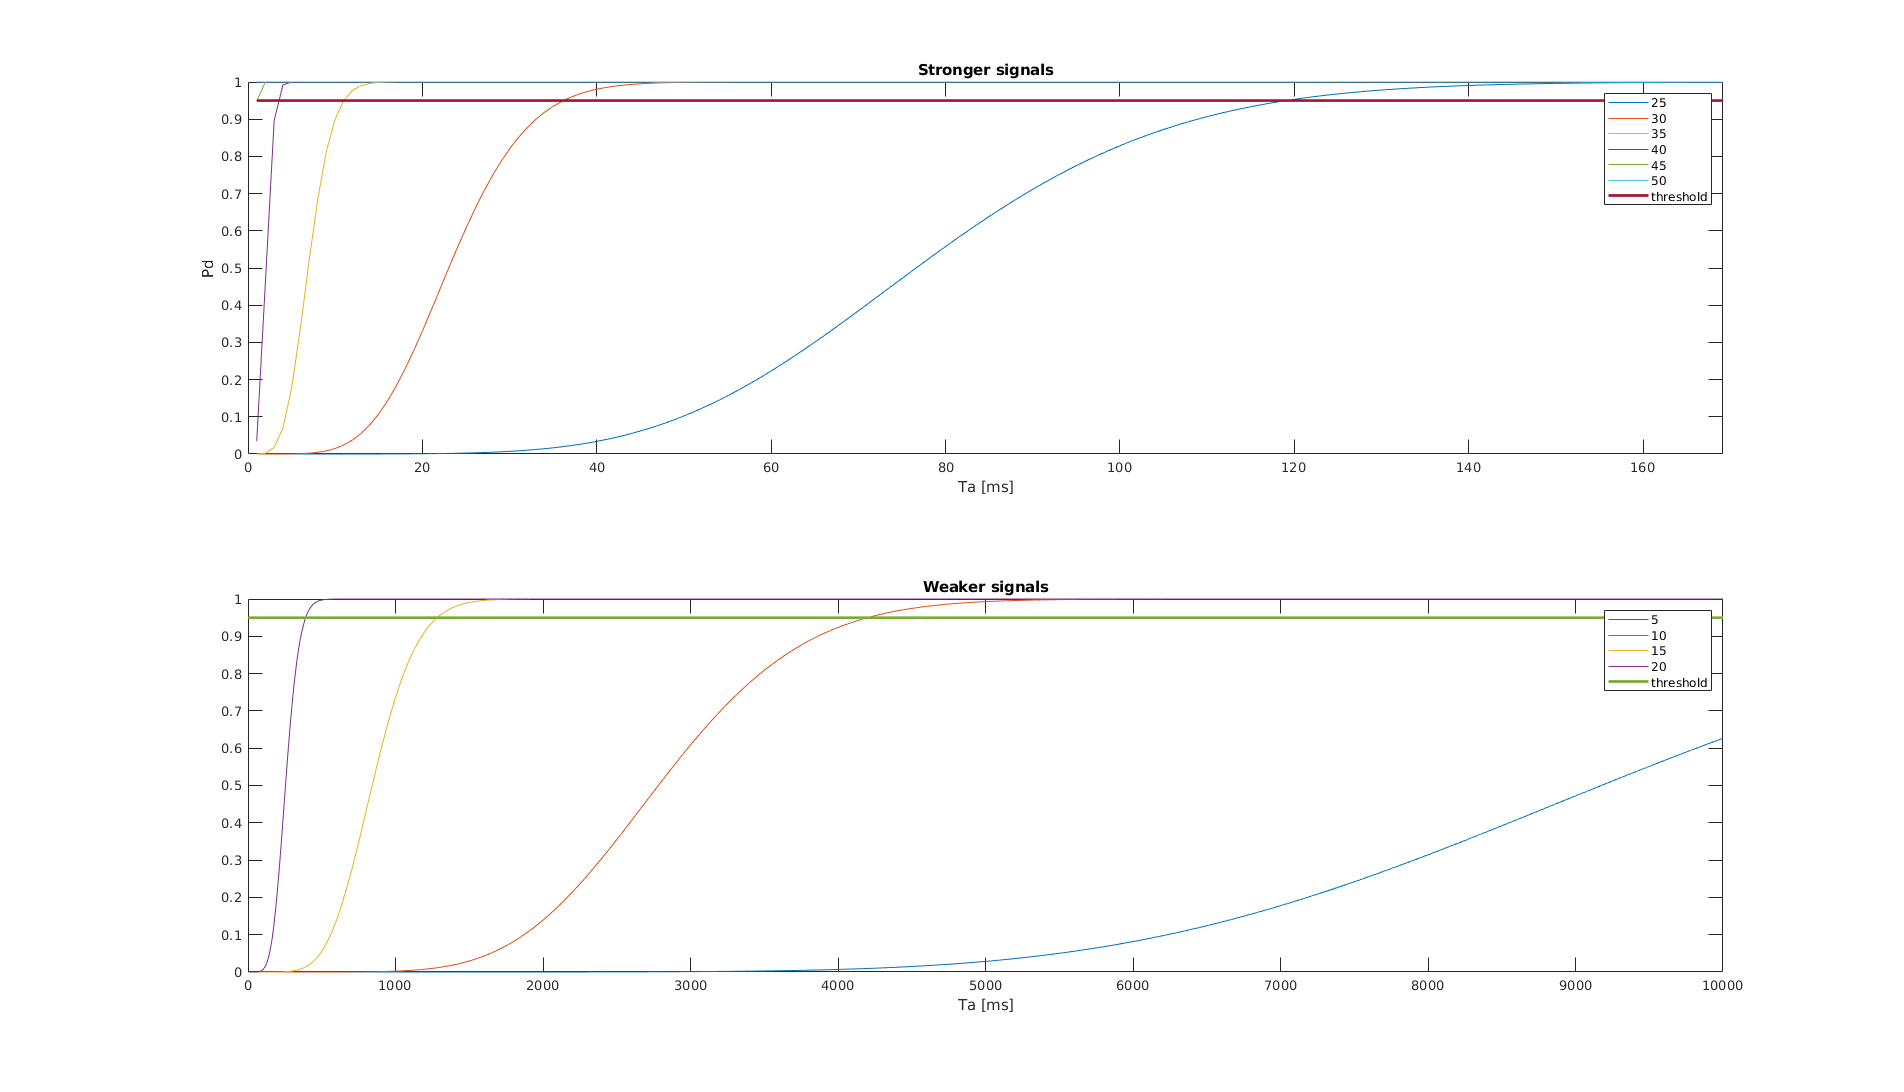
\includegraphics[width=0.9\textwidth]{figs/Pd_vs_Ta.png}
	\caption{Probability of detection vs. accumulation period for
		different C/N0 ratios (Coherent accumulation).}
	\label{fig:pd_vs_Ta}
\end{figure}

In Figure~\ref{fig:HT_partB_30dBHz} it is possible to observe a particular case
of the hypothesis testing for GNSS acquisition. In particular, it is taylored
to detect a 30dBHz C/N0 signal with 95\% probability and 0.01\% chance of false
alarm by performing coherent integration.

\begin{figure}[H]
	\centering
	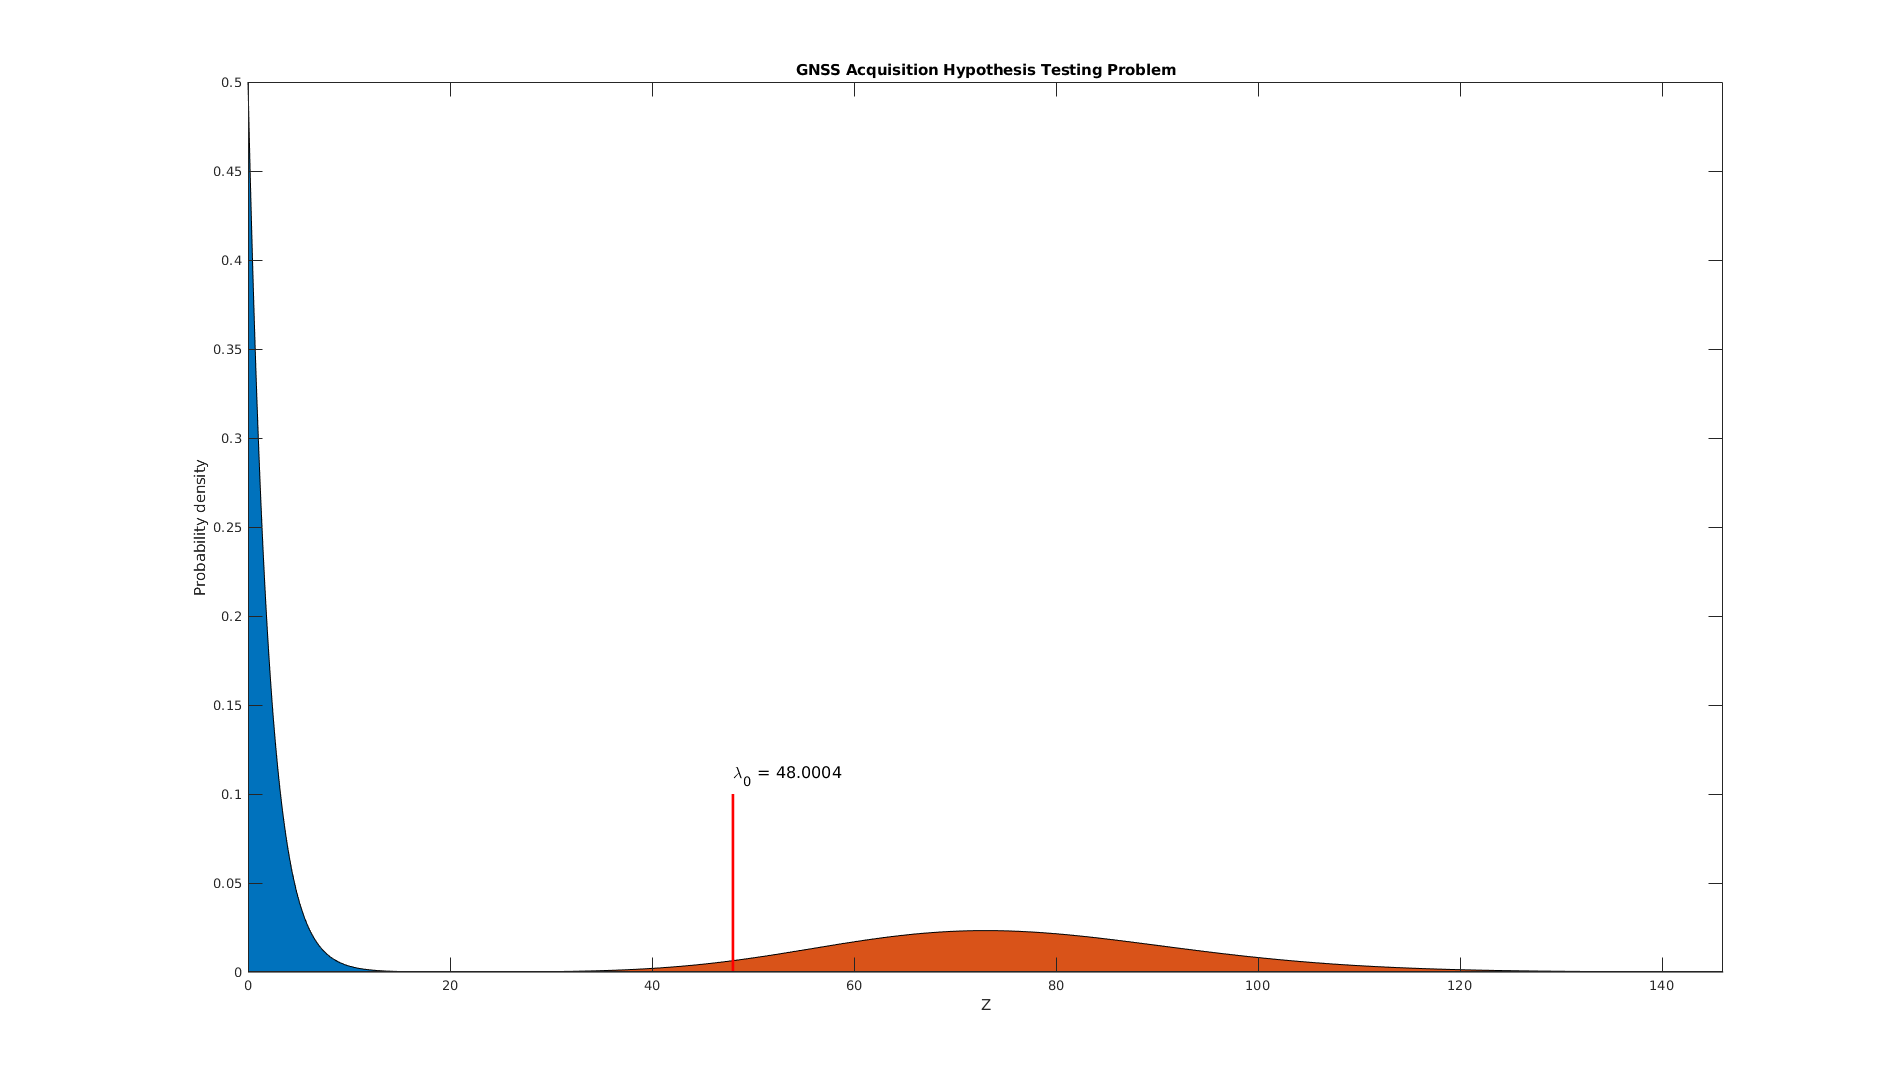
\includegraphics[width=0.9\textwidth]{figs/HT_partB_30dBHz.png}
	\caption{Hypothesis testing for the case where a 30dBHz carrier to noise ratio
		signal. The detection threshold was set to have a probability of false alarm
		0.0001. Then, using $N=1$, $Ta$ was adjusted to get a probability of detection
		greater than 95\%. Thus, $Ta=37ms$.}
	\label{fig:HT_partB_30dBHz}
\end{figure}


Analizing Figure~\ref{fig:HT_partA_30dBHz} and \ref{fig:HT_partB_30dBHz} its is
possible to see that coherent integration leads to a lower overall data usage.
since it needs 37ms of the signal while the non-coherent integration need to
process 99 intervals of 1ms each.


%\bibliographystyle{ieeetr}
%\bibliography{./pangea}  
\end{document}
